\chapter{\textcolor{orange}{SDD - SOFTWARE DESINGN DESCRIPTION}}
%\newpage
%\section{\textcolor{orange}{Historial de Versiones}}
%\begin{table}[!h]
%\begin{center}
%\begin{tabular}{|c|c|c|c|}
%\hline
%\rowcolor[RGB]{255,127,0} Vesión & Fecha & Descripción de Cambios & Autor\\
%\hline
%1.0.0 & 09/07/2013 & Primera Versión del diseño del Sist. & Gomez P.\\
%\hline
%1.0.1 & 12/07/2013 & Descripciòn bàsica de patrones implementados & Lovaisa V.\\
%\hline
%\end{tabular}
%\end{center}
%\end{table}
%\newpage

%\section{\textcolor{orange}{Página de Aprobaciones}}
%A continuación se listan las personas de las cuales se requiere la aceptación de
%cualquier cambio mayor de este documento.
%\begin{enumerate}
  %\item Estas aprobaciones no son necesarias si el cambio es menor.
  %\item Estas aprobaciones son necesarias si el cambio es realizado por alguna
 % persona distinta de ellas.
%\end{enumerate}
%\begin{table}[!h]
%\begin{center}
%\begin{tabular}{|c|c|c|c|}
%\hline
%\rowcolor[RGB]{255,127,0} Nombre & Cargo & Fecha & Firma\\
%\hline
%Lovaisa Valeria & Resp. Diseño & 09/07/2013 & \\
%\hline
%Gomez Pablo & Resp. Suplente & 15/07/2013 & \\
%\hline
%\end{tabular}
%\end{center}
%\end{table}

\newpage
\section{\textcolor{orange}{Introducción}}
\subsection{\textcolor{orange}{Propósito y Alcance}}
Este documento cubre el diseño del sistemade monitoreo y registro de datos multipropósito. Este SDD tiene como objetivo establecer el diseño del sistema , sus componentes , patrones utilizados y lo todo lo relacionado a la etapa de diseño que añada detalles para su implementación. 

\subsection{\textcolor{orange}{Acrónimos y Glosario}}
\begin{table}[!h]
\begin{center}
\begin{tabular}{|c|c|}
\hline
\rowcolor[RGB]{255,127,0} Acrónimo & Descripción \\
\hline
SDD & Software Design Document - Documento de diseño del sistema. \\
\hline
SDM & Software Design Manager – Responsable de diseño del sistema\\
\hline
\end{tabular}
\end{center}
\end{table}

\subsection{\textcolor{orange}{Herramientas Necesarios}}
\begin{table}[!h]
\begin{center}
\begin{tabular}{|c|p{100mm}|}
\hline
\rowcolor[RGB]{255,127,0} Programa & Propósito \\
\hline
Google Driver & Software necesario para llevar los documentos de diseño empleados.\\
%de requermientos usr. vs req. de sistema y de req. vs casos de uso.\\
\hline
Dia & Software para la creación de diagramas UML\\
\hline
Git-Hub & Software necesario para llevar el control de versiones del código \\
\hline
\end{tabular}
\end{center}
\end{table}

%\newpage
%\section{\textcolor{orange}{Roles}}
%\subsection{\textcolor{orange}{Responsables}}

%Las actividades de Diseño del Sistema serán coordinadas en este proyecto por el Responsable de diseño de sistema. (SDM). Este Rol debe ser asignado a alguno de los miembros del proyecto.
%El SDM será el responsable directo de las actividades de diseño, responder ante modificaciones en la misma  y de mantener la documentación relacionada actualizada.


%\subsection{\textcolor{orange}{Roles}}
%\begin{table}[!h]
%\begin{center}
%\begin{tabular}{|c|c|c|}
%\hline
%\rowcolor[RGB]{255,127,0} Rol & Nombre & Suplente\\
%\hline
%SRM & Gomez Pablo & Lovaisa Valeria\\
%\hline
%\end{tabular}
%\end{center}
%\end{table}

\newpage
\section{\textcolor{orange}{Vista general del diseño}}
\subsection{\textcolor{orange}{Diagrama de paquetes}}
% === Figura ====
\begin{figure}[h!]
 \begin{center}
  \includegraphics[width=1\textwidth,keepaspectratio=true]{img/diagrama_paquetes.png}
 %\caption{Flujo de Dato de Temperatura del Sistema}
  \label{fig:esquema}
 \end{center}
\end{figure}
% ===============
%\subsection{\textcolor{orange}{Diagrama de clases paquetes Cliente-Aquisiciòn de Datos}}


\subsection{\textcolor{orange}{Diagrama de clases paquetes Cliente-Presentaciòn de Datos}}


%\subsection{\textcolor{orange}{Diagrama de clases paquetes Servidor}}
% === Figura ====
\begin{figure}[h!]
 \begin{center}
  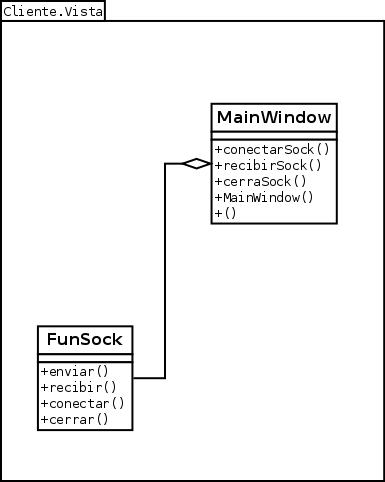
\includegraphics[width=0.5\textwidth,keepaspectratio=true]{img/Clases_Vista.png}
 %\caption{Flujo de Dato de Temperatura del Sistema}
  \label{fig:esquema}
 \end{center}
\end{figure}
% ===============



\section{\textcolor{orange}{Patrones Implementados}}
\subsection{\textcolor{orange}{Patròn Observer }}

Este patrón se utiliza cuando un conjunto de sensores se monitoriza y despliega de manera rutinaria. En el momento en que los sensores indican que sucedió cierto evento, el sistema reacciona iniciando un proceso para manejar dicho evento.
El sensor de temperatura DTH11 rutinariamente toma cada 1seg un nuevo dato de temperatura  y lo envía a través de una interfaz Ethernet a un servidor

\subsection{\textcolor{orange}{Patrón Ambiental}}

Este patrón se emplea cuando un sistema incluye sensores que proporcionan información sobre el entorno y los actuadores que pueden cambiar el entorno. En respuesta a los cambios ambientales detectados por el sensor, se envían señales de control a los actuadores del sistema.

El sensor de temperatura toma la temperatura del el entorno y el servidor verifica que los valores medidos se encuentren dentro de el rango establecido, en el caso de no cumplir con los valores mínimos y máximos de temperatura pre establecidos el servidor lanza una alarma que se puede visualizar en el monitor conectado en de la terminal de la plataforma hardware iMx53.

 
\subsection{\textcolor{orange}{Segmentaciòn de Proceso(process pipeline)}}

Este patrón se usa al transformarse datos de una representación a otra antes de que puedan procesarse. La transformación se implementa como una secuencia de pasos de procesamiento, que puede realizarse de manera concurrente. Esto permite un procesamiento de datos muy rápido, debido a un núcleo o procesador separado puede ejecutar cada transformación.

El proceso productor en el servidor recibe por medio de la interfaz Ethernet el dato de temperatura y lo graba en un buffer circular en memoria compartida donde el proceso consumidor toma el dato lo procesa, lo registra en una base de datos y lo envía a través de la interfaz Ethernet para ser presentado

